% =========================================================================
%  P-TRANSMIT AI - Beamer deck (compile on Overleaf, pdfLaTeX)
%  Title: Artificial Intelligence for Malaria Transmission Intelligence
%  Branding: KCCR - KNUST, Kumasi, Ghana
%  Graphics: PNG logos at 300+ dpi => crisp, high-resolution PDF output
% =========================================================================
\documentclass[aspectratio=169,11pt]{beamer}

% ---------- Brand palette (Ghana / KNUST) --------------------------------
\definecolor{knustred}{HTML}{8F141B}
\definecolor{ggreen}{HTML}{0B6E4F}
\definecolor{ggold}{HTML}{D4A017}
\definecolor{navy}{HTML}{0D1F2D}
\definecolor{slate}{HTML}{5A6B76}
\definecolor{paper}{HTML}{FFFFFF}
\definecolor{mist}{HTML}{EEF1F3}

\usepackage[T1]{fontenc}
\usepackage{lmodern}          % scalable vector fonts (sharp at any zoom)
\usepackage{microtype}        % better glyph placement
\usepackage{graphicx}
\usepackage{booktabs}
\usepackage{tikz}
\usetikzlibrary{positioning,arrows.meta,backgrounds,calc}
\usepackage{pgfplots}
\pgfplotsset{compat=1.17}

% ---------- Beamer theme --------------------------------------------------
\usetheme{Madrid}
\useinnertheme{circles}
\setbeamercolor{structure}{fg=ggreen}
\setbeamercolor{palette primary}{bg=ggreen,fg=white}
\setbeamercolor{palette secondary}{bg=navy,fg=white}
\setbeamercolor{palette tertiary}{bg=knustred,fg=white}
\setbeamercolor{frametitle}{bg=navy,fg=white}
\setbeamercolor{title}{bg=navy,fg=white}
\setbeamercolor{block title}{bg=ggreen,fg=white}
\setbeamercolor{block body}{bg=mist,fg=black}
\setbeamercolor{alertblock title}{bg=knustred,fg=white}
\setbeamercolor{alertblock body}{bg=knustred!8,fg=black}
\setbeamercolor{block title alerted}{bg=knustred,fg=white}
\setbeamercolor{itemize item}{fg=ggold}
\setbeamercolor{itemize subitem}{fg=ggreen}
\setbeamercolor{enumerate item}{fg=knustred}
\setbeamerfont{frametitle}{series=\bfseries,size=\large}
\setbeamertemplate{navigation symbols}{}
\setbeamertemplate{footline}[frame number]

% Ghana tricolour footline accent
\addtobeamertemplate{footline}{}{%
  \hfill%
  
\begin{tikzpicture}[baseline]
    \fill[ggreen] (0,0) rectangle (0.28,0.07);
    \fill[ggold]  (0.30,0) rectangle (0.58,0.07);
    \fill[knustred] (0.60,0) rectangle (0.88,0.07);
  \end{tikzpicture}\hspace{2pt}}

% ---------- Logos ---------------------------------------------------------
% Put these files next to main.tex (Overleaf: upload to project root)
\newif\iflogos
\IfFileExists{kccr_knust.png}{\logostrue}{\logosfalse}

\newcommand{\BrandBar}{%
  \iflogos
    \begin{tikzpicture}[baseline]
      \node[anchor=west,inner sep=0] (a) at (0,0)
        {\includegraphics[height=0.62cm]{kccr_knust.png}};
      \draw[slate!40] (2.35,0.02) -- (2.35,0.6);
      \node[anchor=west,text=slate,font=\tiny\bfseries] at (2.5,0.3)
        {KCCR~$\cdot$~KNUST\ \ MALARIA AI SEMINAR};
    \end{tikzpicture}%
  \else
    {\tiny\bfseries\textcolor{slate}{KCCR~$\cdot$~KNUST\ \ MALARIA AI SEMINAR}}%
  \fi}

\addtobeamertemplate{frametitle}{}{%
  \begin{tikzpicture}[remember picture,overlay]
    \node[anchor=north east,yshift=-2pt,xshift=-4pt] at (current page.north east) {\BrandBar};
  \end{tikzpicture}}

% ---------- Title page ----------------------------------------------------
\title[AI for Malaria Transmission Intelligence]{Artificial Intelligence for\\ \textcolor{ggold}{Malaria Transmission} Intelligence}
\subtitle{From \emph{Plasmodium} biology to machine-learning surveillance:\\the P-TRANSMIT AI platform for Ghana's elimination agenda}
\author[[Your Name]]{[Your Name]}
\institute[KCCR $\cdot$ KNUST]{Kumasi Centre for Collaborative Research in Tropical Medicine\\Kwame Nkrumah University of Science and Technology, Kumasi}
\date{Research Seminar $\cdot$ September 2026}

\begin{document}

% ======================= 1 - TITLE =======================================
\begin{frame}[plain]
  \titlepage
  \vspace{-4mm}
  \begin{center}
    \iflogos
      \includegraphics[height=1.15cm]{kccr_knust.png}\hspace{14mm}%
      \includegraphics[height=1.2cm]{knust_seal}\hspace{10mm}%
      {\footnotesize\textcolor{slate}{Kumasi Centre for Collaborative Research $\cdot$ KNUST $\cdot$ Ghana}}
    \fi
  \end{center}
\end{frame}

% ======================= 2 - OUTLINE =====================================
\begin{frame}{What we will cover}
  \small
  \begin{columns}[t]
    \column{0.48\textwidth}
    \begin{enumerate}
      \item The malaria problem in Ghana
      \item \emph{Plasmodium}: the parasite
      \item Transmission dynamics
      \item Why AI, why now
      \item AI in transmission studies: adoption
      \item Data foundations
    \end{enumerate}
    \column{0.48\textwidth}
    \begin{enumerate}\setcounter{enumi}{6}
      \item The P-TRANSMIT AI platform
      \item Transmission forecasting engine
      \item Spatial intelligence and early warning
      \item Genomics and resistance guardrails
      \item Responsible AI
      \item Roadmap and close
    \end{enumerate}
  \end{columns}
\end{frame}

% ======================= 3 - MALARIA IN GHANA ============================
\begin{frame}{Malaria in Ghana: a persistent national burden}
  \begin{columns}[c]
    \begin{column}{0.52\textwidth}
      \begin{block}{Where we stand}
        \begin{itemize}
          \item Endemic in all 16 regions; the whole country carries risk
          \item Roughly five million suspected cases tested every year
          \item A top-three reason for outpatient attendance nationwide
          \item Children under five and pregnant women bear the worst outcomes
        \end{itemize}
      \end{block}
      \begin{alertblock}{Why it persists}
        Year-round transmission in the south, sharp seasonal peaks up north, and
        moving targets: insecticide resistance, \emph{pfhrp2/3} deletions,
        emerging artemisinin markers.
      \end{alertblock}
    \end{column}
    \begin{column}{0.44\textwidth}
      \centering
      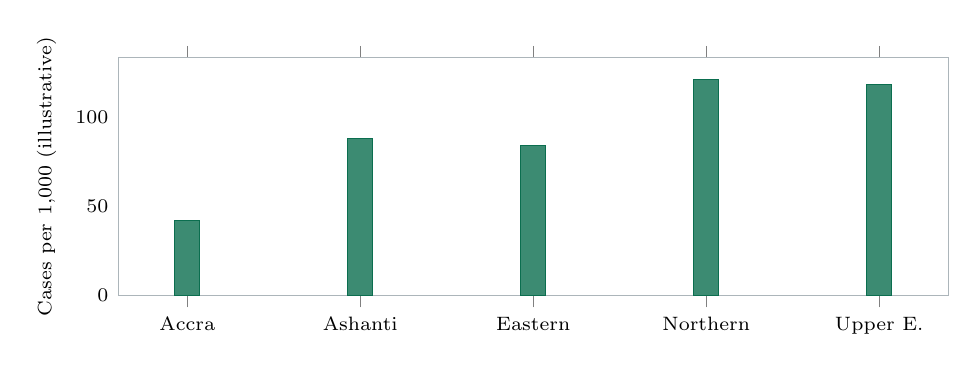
\begin{tikzpicture}
        \begin{axis}[
          width=\textwidth, height=4.6cm,
          ybar, bar width=9pt,
          symbolic x coords={Accra,Ashanti,Eastern,Northern,Upper E.},
          xtick=data, ymin=0,
          ylabel={Cases per 1{,}000 (illustrative)},
          axis line style={slate!50}, tick label style={font=\scriptsize},
          label style={font=\scriptsize}, ytick style={draw=none},
          nodes near coords style={font=\tiny},
        ]
          \addplot[fill=ggreen!80,draw=ggreen] coordinates
            {(Accra,42) (Ashanti,88) (Eastern,84) (Northern,121) (Upper E.,118)};
        \end{axis}
      \end{tikzpicture}\\
      {\scriptsize\textcolor{slate}{Illustrative regional intensity (synthetic demo values).}}
      \vspace{2mm}
      \begin{block}{What elimination demands}
        Forward-looking, region-level forecasting. Not retrospective reporting.
      \end{block}
    \end{column}
  \end{columns}
\end{frame}

% ======================= 4 - PLASMODIUM ==================================
\begin{frame}{\emph{Plasmodium}: four species, one disease burden}
  \small
  \begin{columns}[c]
    \begin{column}{0.62\textwidth}
      \begin{table}
        \begin{tabular}{@{}p{1.9cm}p{2.6cm}p{3.4cm}@{}}
          \toprule
          \textbf{Species} & \textbf{Role in Ghana} & \textbf{Key trait} \\
          \midrule
          \emph{P. falciparum} & Dominant, over 95\% of cases & Severe disease, cytoadherence \\
          \emph{P. vivax} & Rare in Ghana & Dormant liver stages, relapses \\
          \emph{P. malariae} & Low, often co-infections & Chronic low-grade parasitaemia \\
          \emph{P. ovale} & Sparse, coastal & Hypnozoite relapses, mild \\
          \bottomrule
        \end{tabular}
      \end{table}
      \begin{block}{A compact genome}
        About 23 megabases across 14 chromosomes and roughly 5{,}300 genes.
        Small enough for full population-genomic surveillance, large enough to
        hide resistance and immune-evasion variants.
      \end{block}
    \end{column}
    \begin{column}{0.34\textwidth}
      \begin{block}{Two-host life cycle}
        \begin{center}
        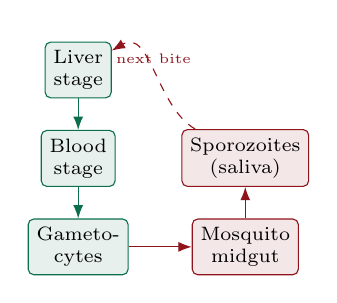
\begin{tikzpicture}[node distance=4mm,every node/.style={font=\scriptsize,align=center},
                           box/.style={draw=ggreen,fill=ggreen!10,rounded corners=2pt,inner sep=3pt}]
          \node[box] (l) {Liver\\stage};
          \node[box,below=of l] (b) {Blood\\stage};
          \node[box,below=of b] (g) {Gameto-\\cytes};
          \node[box,right=8mm of g,fill=knustred!10,draw=knustred] (m) {Mosquito\\midgut};
          \node[box,above=of m,fill=knustred!10,draw=knustred] (s) {Sporozoites\\(saliva)};
          \draw[-{Latex},ggreen] (l)--(b); \draw[-{Latex},ggreen] (b)--(g);
          \draw[-{Latex},knustred] (g)--(m); \draw[-{Latex},knustred] (m)--(s);
          \draw[-{Latex},knustred,dashed] (s) to[out=150,in=30] node[above,font=\tiny]{next bite} (l);
        \end{tikzpicture}
        \end{center}
      \end{block}
    \end{column}
  \end{columns}
\end{frame}

% ======================= 5 - TRANSMISSION DYNAMICS =======================
\begin{frame}{Transmission is a spatiotemporal system}
  \centering
  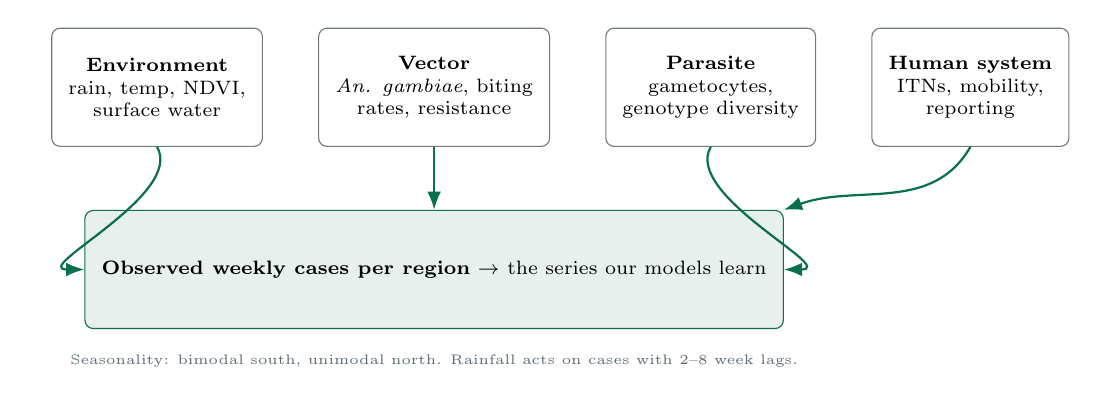
\begin{tikzpicture}[every node/.style={font=\scriptsize,align=center},
      stage/.style={draw=navy!60,fill=white,rounded corners=3pt,inner sep=6pt,minimum width=2.5cm,minimum height=1.5cm}]
    \node[stage] (env) {\textbf{Environment}\\rain, temp, NDVI,\\surface water};
    \node[stage,right=7mm of env] (vec) {\textbf{Vector}\\\emph{An. gambiae}, biting\\rates, resistance};
    \node[stage,right=7mm of vec] (par) {\textbf{Parasite}\\gametocytes,\\genotype diversity};
    \node[stage,right=7mm of par] (hum) {\textbf{Human system}\\ITNs, mobility,\\reporting};
    \node[stage,below=8mm of vec,fill=ggreen!10,draw=ggreen,minimum width=6.5cm] (out)
      {\textbf{Observed weekly cases per region} $\rightarrow$ the series our models learn};
    \draw[-{Latex},thick,ggreen] (env.south) to[out=-60,in=180] (out.west);
    \draw[-{Latex},thick,ggreen] (vec.south) -- (out.north);
    \draw[-{Latex},thick,ggreen] (par.south) to[out=-120,in=0] (out.east);
    \draw[-{Latex},thick,ggreen] (hum.south) to[out=-120,in=20] (out.north east);
    \node[font=\tiny,text=slate,below=2mm of out]
      {Seasonality: bimodal south, unimodal north. Rainfall acts on cases with 2--8 week lags.};
  \end{tikzpicture}
  \vfill
  \begin{columns}[c]
    \begin{column}{0.48\textwidth}
      \begin{block}{Lags are everything}
        Rain to breeding sites to adult mosquitoes to infection to case: about
        two to eight weeks. Models that respect these lags win.
      \end{block}
    \end{column}
    \begin{column}{0.48\textwidth}
      \begin{block}{What this means for AI}
        Any serious model must fuse case history, environment and seasonality
        for all regions at once. That is exactly what machine learning is good at.
      \end{block}
    \end{column}
  \end{columns}
\end{frame}

% ======================= 6 - WHY AI ======================================
\begin{frame}{Why AI, why now}
  \begin{columns}[c]
    \begin{column}{0.32\textwidth}
      \begin{block}{Classical models}
        \begin{itemize}\small
          \item Ross--Macdonald: elegant, interpretable
          \item Parameters costly and slow to measure
          \item Struggle with sparse routine data
        \end{itemize}
      \end{block}
    \end{column}
    \begin{column}{0.32\textwidth}
      \begin{alertblock}{What ML adds}
        \begin{itemize}\small
          \item Learns lags and thresholds from data
          \item Blends cases, climate, mobility, genomics
          \item Covers all 16 regions, updated weekly
        \end{itemize}
      \end{alertblock}
    \end{column}
    \begin{column}{0.32\textwidth}
      \begin{block}{Decision value}
        \begin{itemize}\small
          \item Pre-position RDTs, drugs, IRS before peaks
          \item Prioritise districts for vector control
          \item Early signals trigger field investigation
        \end{itemize}
      \end{block}
    \end{column}
  \end{columns}
  \vspace{3mm}
  \begin{block}{A caution we take seriously}
    Models learn associations in the data they are given. Garbage in, garbage
    out. Data quality, honest validation and human review are not optional.
    P-TRANSMIT AI is engineered around this principle.
  \end{block}
\end{frame}

% ======================= 7 - ADOPTION LANDSCAPE ==========================
\begin{frame}{Adoption of AI in malaria transmission studies}
  \begin{columns}[c]
    \begin{column}{0.55\textwidth}
      \centering
      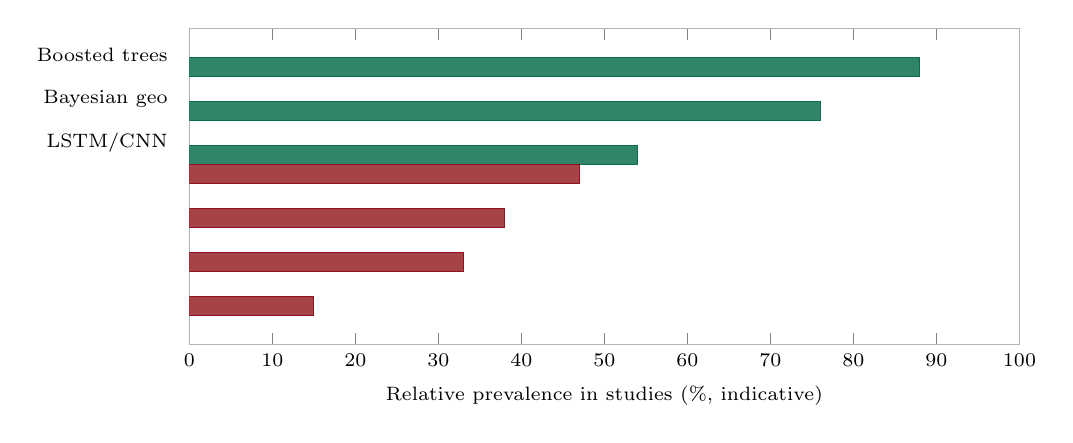
\begin{tikzpicture}
        \begin{axis}[
          width=\textwidth, height=5.6cm, xbar, bar width=7pt,
          symbolic y coords={LLM-assisted,Genomic ML,Hybrid ML+mech,Imagery CNNs,LSTM/CNN,Bayesian geo,Boosted trees},
          ytick=data,
          xmin=0,xmax=100,
          xlabel={Relative prevalence in studies (\%, indicative)},
          axis line style={slate!50}, tick label style={font=\scriptsize},
          label style={font=\scriptsize}, ytick style={draw=none},
        ]
          \addplot[fill=ggreen!85,draw=ggreen] coordinates
            {(88,Boosted trees) (76,Bayesian geo) (54,LSTM/CNN)};
          \addplot[fill=knustred!80,draw=knustred] coordinates
            {(47,Imagery CNNs) (38,Hybrid ML+mech) (33,Genomic ML) (15,LLM-assisted)};
        \end{axis}
      \end{tikzpicture}\\
      {\scriptsize\textcolor{slate}{Indicative synthesis of 2015--2025 literature; exact shares vary by review.}}
    \end{column}
    \begin{column}{0.42\textwidth}
      \begin{block}{Established}
        Risk mapping in the Malaria Atlas Project style, seasonal outbreak
        forecasting, climate-driven early warning.
      \end{block}
      \begin{alertblock}{Accelerating}
        DHIS2-linked dashboards, drone and CNN larval surveys, mobility
        features, marker trend models.
      \end{alertblock}
      \begin{block}{Persistent gaps}
        Few deployable African-built platforms, weak documentation, rare
        external validation. P-TRANSMIT targets exactly these gaps.
      \end{block}
    \end{column}
  \end{columns}
\end{frame}

% ======================= 8 - DATA FOUNDATIONS ============================
\begin{frame}{Five data streams, one disciplined pipeline}
  \begin{columns}[c]
    \begin{column}{0.63\textwidth}
      \small
      \begin{itemize}
        \item \textbf{Surveillance}: weekly confirmed cases per region. The target variable.
        \item \textbf{Environmental}: rainfall, temperature, NDVI (CHIRPS, ERA5, MODIS). Leading indicators.
        \item \textbf{Genomic}: variant calls and marker tables from KCCR pipelines.
        \item \textbf{Resistance}: marker frequencies plus treatment outcomes (SMART-style protocols).
        \item \textbf{Spatial}: geoBoundaries ADM1/ADM2, WorldPop denominators.
      \end{itemize}
    \end{column}
    \begin{column}{0.33\textwidth}
      \begin{alertblock}{Pipeline discipline}
        Automatic profiling, missingness reports, fuzzy region matching, explicit
        column mapping. Nothing is imputed silently, and synthetic data stays
        permanently flagged.
      \end{alertblock}
    \end{column}
  \end{columns}
  \vspace{2mm}
  \begin{block}{Feature engineering, the transmission lens}
    Case lags 1--4 weeks, rolling means, rainfall and temperature at lags 2--8
    weeks, week-of-year harmonics, region identifiers, population-normalised
    rates. Every feature is documented, versioned and auditable.
  \end{block}
\end{frame}

% ======================= 9 - PLATFORM OVERVIEW ===========================
\begin{frame}{P-TRANSMIT AI: one platform, ten modules}
  \small
  \begin{columns}[c]
    \begin{column}{0.32\textwidth}
      \begin{block}{\textbf{Dashboard}}\scriptsize National KPIs, risk map, forecast bars, explainability.\end{block}
      \begin{block}{\textbf{Transmission AI}}\scriptsize Train and forecast weekly cases at 1/2/4/8-week horizons.\end{block}
      \begin{block}{\textbf{Spatial Intelligence}}\scriptsize Interactive choropleth: risk, observed cases, forecast medians.\end{block}
    \end{column}
    \begin{column}{0.32\textwidth}
      \begin{block}{\textbf{Genomics}}\scriptsize Marker tables, regional frequencies, AMR charts.\end{block}
      \begin{block}{\textbf{Resistance}}\scriptsize SMART-style surveillance scaffolding with guardrails.\end{block}
      \begin{block}{\textbf{Early Warning}}\scriptsize Signals with evidence, severity and a review workflow.\end{block}
    \end{column}
    \begin{column}{0.32\textwidth}
      \begin{block}{\textbf{Data Explorer}}\scriptsize Upload CSV, Excel or JSON; quality profiling; fuzzy matching.\end{block}
      \begin{block}{\textbf{Model Laboratory}}\scriptsize Model zoo, seeds, temporal validation, provenance.\end{block}
      \begin{block}{\textbf{Reports}}\scriptsize One-click reproducibility-oriented markdown reports.\end{block}
    \end{column}
  \end{columns}
  \vspace{2mm}
  \centering
  \begin{alertblock}{}
    Locally hosted (FastAPI + React). Every prediction ships with provenance,
    metrics and explicit limitations.
  \end{alertblock}
\end{frame}

% ======================= 10 - ENGINE =====================================
\begin{frame}{Transmission forecasting: how the AI actually works}
  \centering
  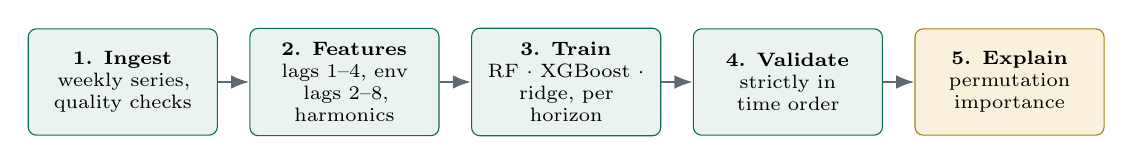
\begin{tikzpicture}[every node/.style={font=\scriptsize,align=center},
      st/.style={draw=ggreen,fill=ggreen!8,rounded corners=3pt,inner sep=5pt,minimum height=1.35cm,text width=2.05cm}]
    \node[st] (s1) {\textbf{1. Ingest}\\weekly series,\\quality checks};
    \node[st,right=4mm of s1] (s2) {\textbf{2. Features}\\lags 1--4, env\\lags 2--8, harmonics};
    \node[st,right=4mm of s2] (s3) {\textbf{3. Train}\\RF $\cdot$ XGBoost $\cdot$\\ridge, per horizon};
    \node[st,right=4mm of s3] (s4) {\textbf{4. Validate}\\strictly in\\time order};
    \node[st,right=4mm of s4,fill=ggold!15,draw=ggold!80!black] (s5) {\textbf{5. Explain}\\permutation\\importance};
    \draw[-{Latex},thick,slate] (s1)--(s2); \draw[-{Latex},thick,slate] (s2)--(s3);
    \draw[-{Latex},thick,slate] (s3)--(s4); \draw[-{Latex},thick,slate] (s4)--(s5);
  \end{tikzpicture}
  \vspace{3mm}
  \begin{columns}[c]
    \begin{column}{0.32\textwidth}\centering
      {\Large\textcolor{ggreen}{\textbf{3}}}\\ model families\\ {\scriptsize trees, boosting, ridge}
    \end{column}
    \begin{column}{0.32\textwidth}\centering
      {\Large\textcolor{ggold!80!black}{\textbf{4}}}\\ forecast horizons\\ {\scriptsize +1, +2, +4, +8 weeks}
    \end{column}
    \begin{column}{0.32\textwidth}\centering
      {\Large\textcolor{knustred}{\textbf{0}}}\\ random leakage tolerated\\ {\scriptsize time walks forward only}
    \end{column}
  \end{columns}
  \vspace{2mm}
  \begin{block}{Demo metrics (synthetic data)}
    Held-out MAE about 5 to 9 weekly cases per region across horizons. Models
    stay honest: MAE and RMSE are reported on weeks the model never saw.
  \end{block}
\end{frame}

% ======================= 11 - SPATIAL + ALERTS ===========================
\begin{frame}{Spatial intelligence and early-warning signals}
  \begin{columns}[c]
    \begin{column}{0.48\textwidth}
      \begin{block}{Interactive risk cartography}
        \begin{itemize}\small
          \item Leaflet choropleth of all 16 regions (geoBoundaries ADM1, CC-BY 4.0)
          \item Three layers: risk category, recent 4-week mean, forecast median
          \item Risk classes come from each dataset's own history
        \end{itemize}
      \end{block}
    \end{column}
    \begin{column}{0.48\textwidth}
      \begin{alertblock}{Early-warning workflow}
        \begin{itemize}\small
          \item Scan compares recent weeks to the historical 90th percentile
          \item Every signal carries evidence, severity and a model reference
          \item Humans acknowledge or dismiss; the system never acts alone
        \end{itemize}
      \end{alertblock}
    \end{column}
  \end{columns}
  \vspace{2mm}
  \begin{block}{Live demo numbers (synthetic scenario)}
    The scripted demonstration includes a late-season upswing in the Northern,
    Upper East, Ashanti and Greater Accra regions, which triggers 9 research
    signals and lifts several regions into elevated risk categories on the map.
  \end{block}
\end{frame}

% ======================= 12 - GENOMICS ===================================
\begin{frame}{\emph{Plasmodium} genomics and resistance guardrails}
  \begin{columns}[c]
    \begin{column}{0.48\textwidth}
      \begin{block}{Genomics module}
        \begin{itemize}\small
          \item Marker calls by gene, watchlist share by region
          \item Marker-positive share over time (kelch13, pfdhps, pfcrt, pfmdr1)
          \item Most frequent mutations at a glance
          \item Phase 2: heterozygosity, MOI, population structure
        \end{itemize}
      \end{block}
    \end{column}
    \begin{column}{0.48\textwidth}
      \begin{block}{Resistance module}
        \begin{itemize}\small
          \item SMART-style surveillance scaffolding
          \item Catalogue: \emph{kelch13}, \emph{pfcrt}, \emph{pfmdr1}, \emph{pfdhfr/pfdhps}, \emph{pfhrp2/3}
          \item Outcome-data integration where ethically approved
        \end{itemize}
      \end{block}
    \end{column}
  \end{columns}
  \vspace{2mm}
  \begin{alertblock}{The bright line}
    A detected genetic marker is \textbf{not} phenotypic drug resistance.
    Interpretation thresholds are researcher-supplied, from WHO or published
    definitions. The platform never invents them.
  \end{alertblock}
\end{frame}

% ======================= 13 - RESPONSIBLE AI =============================
\begin{frame}{Governance is engineered, not appended}
  \begin{columns}[c]
    \begin{column}{0.48\textwidth}
      \begin{block}{Scientific honesty}
        \begin{itemize}\small
          \item Synthetic demonstration data stays permanently labelled
          \item Temporal validation only; MAE and RMSE lead, $R^2$ for completeness
          \item Intervals are residual-based, and we say so
          \item Every model stored with dataset, features, seed and versions
        \end{itemize}
      \end{block}
    \end{column}
    \begin{column}{0.48\textwidth}
      \begin{block}{Human primacy}
        \begin{itemize}\small
          \item Every screen: predictions are not diagnoses
          \item Alerts need a human to acknowledge or dismiss
          \item Role-based access and full audit logs
          \item No personal identifiers in uploads
        \end{itemize}
      \end{block}
    \end{column}
  \end{columns}
  \vspace{2mm}
  \begin{columns}[c]
    \begin{column}{0.32\textwidth}\begin{block}{Provenance}\scriptsize Full lineage from uploaded file to forecast row.\end{block}\end{column}
    \begin{column}{0.32\textwidth}\begin{block}{Equity}\scriptsize Region-relative risk avoids punishing low-reporting districts.\end{block}\end{column}
    \begin{column}{0.32\textwidth}\begin{block}{Reproducibility}\scriptsize One-click report regenerates the full analysis trail.\end{block}\end{column}
  \end{columns}
\end{frame}

% ======================= 14 - ROADMAP ====================================
\begin{frame}{Deployment roadmap}
  \begin{columns}[c]
    \begin{column}{0.32\textwidth}
      \begin{block}{Phase 1: now, complete}
        \begin{itemize}\scriptsize
          \item Data Explorer with quality profiling
          \item Forecasting engine, 3 models by 4 horizons
          \item Spatial dashboard and alert scan
          \item Auth, audit logs, provenance, reports
        \end{itemize}
      \end{block}
    \end{column}
    \begin{column}{0.32\textwidth}
      \begin{alertblock}{Phase 2: 3--6 months}
        \begin{itemize}\scriptsize
          \item KCCR genomic connector (data agreement)
          \item MOI, heterozygosity, structure analytics
          \item Marker trends with researcher-set thresholds
          \item LSTM evaluation, probabilistic intervals
        \end{itemize}
      \end{alertblock}
    \end{column}
    \begin{column}{0.32\textwidth}
      \begin{block}{Phase 3: 6--18 months}
        \begin{itemize}\scriptsize
          \item CHIRPS, ERA5, NDVI automated ingestion
          \item Environmental-suitability map layers
          \item District-level (ADM2) resolution
          \item Prospective evaluation with NMCP, Ashanti pilot
        \end{itemize}
      \end{block}
    \end{column}
  \end{columns}
  \vspace{2mm}
  \begin{exampleblock}{North star}
    A nationally trusted, locally hosted AI surveillance companion that
    shortens the distance from data to signal to field action. Built in Ghana,
    by Ghanaian institutions, for the elimination agenda.
  \end{exampleblock}
\end{frame}

% ======================= 15 - CLOSING ====================================
\begin{frame}{AI is now practical infrastructure for malaria intelligence}
  \begin{block}{Three things to remember}
    \begin{enumerate}
      \item Transmission is spatiotemporal. Models must respect time, space and lags.
      \item Markers are not resistance, and predictions are not diagnoses. Guardrails make AI usable in public health.
      \item Local ownership matters: locally hosted, locally governed, built for Ghana's workflows.
    \end{enumerate}
  \end{block}
  \vspace{3mm}
  \begin{block}{Acknowledgements}
    Kumasi Centre for Collaborative Research in Tropical Medicine (KCCR).
    Kwame Nkrumah University of Science and Technology (KNUST).
    Ghana NMCP and regional health directorates as Phase 3 data partners.
  \end{block}
  \vfill
  \centering{\large Questions and a live demonstration are welcome.}\\[1mm]
  {\scriptsize\textcolor{slate}{Platform: \texttt{http://localhost:4173}}}
\end{frame}

\end{document}
